\chapter{Implementation}

This chapter details the core implementation components of the agentic AI framework, including web scraping for knowledge acquisition, vector database construction for factual grounding, and the multi-agent workflow orchestrated with LangGraph.

\section{Web Scraping and Data Collection}

To build a comprehensive, up-to-date knowledge base of cloud documentation, a custom web scraping pipeline was developed in Python. The process involves:

\begin{itemize}
\item \textbf{Target Resource Identification:} The system targets official AWS documentation URLs such as \url{https://docs.aws.amazon.com/}
 and \url{https://docs.aws.amazon.com/en_us/main-landing-page.xml}
, specifically focusing on core service documentation and whitepapers.
\item \textbf{Link Extraction:} Using the \texttt{requests} and \texttt{BeautifulSoup} libraries, the scraper extracts service-specific links and filters for relevant whitepapers, developer guides, and official PDFs.
\item \textbf{PDF Discovery and Metadata Retrieval:} The scraper probes for the presence of guide-info JSON metadata files (e.g., \texttt{meta-inf/guide-info.json}) at multiple subpaths, following redirects to retrieve direct links to PDF documents.
\item \textbf{Manual Search:} Documentation was manually reviewed to identify and include missing core services.
\item \textbf{Storage:} Discovered URLs are deduplicated, metadata-tagged, and stored in a structured CSV dataset for downstream processing.
\end{itemize}

This automated data ingestion pipeline ensures the knowledge base reflects the latest cloud offerings and best practices, which are crucial for factual validation.

\section{Vector Database Construction}

The collected documentation PDFs are processed and embedded into a vector index to facilitate rapid semantic retrieval. Key steps include:

\begin{itemize}
\item \textbf{Document Parsing:} Using the \texttt{Docling} toolkit \cite{docling2025paper}, complex PDFs are parsed into clean, structured text. The parser handles tables, images, and multi-column layouts.
\item \textbf{Pre processing:} The data is preprocessed by converting PDFs to Markdown and then removing elements such as images, irrelevant tables, and other non-vectorizable content.
\item \textbf{Text Chunking:} The parsed content is split into semantically meaningful chunks using the \texttt{MarkdownHeaderTextSplitter} and \\
\texttt{RecursiveCharacterTextSplitter} from the LangChain framework, respecting chunk size and overlap constraints.
\item \textbf{Embedding Generation:} The \texttt{Nomic-embed-text} model served via Ollama \cite{ollama2024web} generates dense vector embeddings for each chunk. These embeddings capture semantic meaning, enabling similarity-based retrieval.
\item \textbf{Vector Indexing with ChromaDB:} The embeddings are stored in the open-source ChromaDB vector database \cite{chromadb2024}, optimized for scalable similarity search. Each document chunk retains metadata (source URL, service, domain), enabling context-aware retrieval.
\end{itemize}

The resulting vector store underpins the validation process, ensuring factual grounding of generated solutions.

\section{Agentic Workflow}

The system is implemented as a cyclic multi-agent graph managed by LangGraph \cite{langgraph2024docs}.

The complete orchestration of these agents, including the conditional edges and feedback loops, is visualized in the graph structure generated by LangGraph, as shown in Figure \ref{fig:langgraph}.

\begin{figure}[H]
\centering
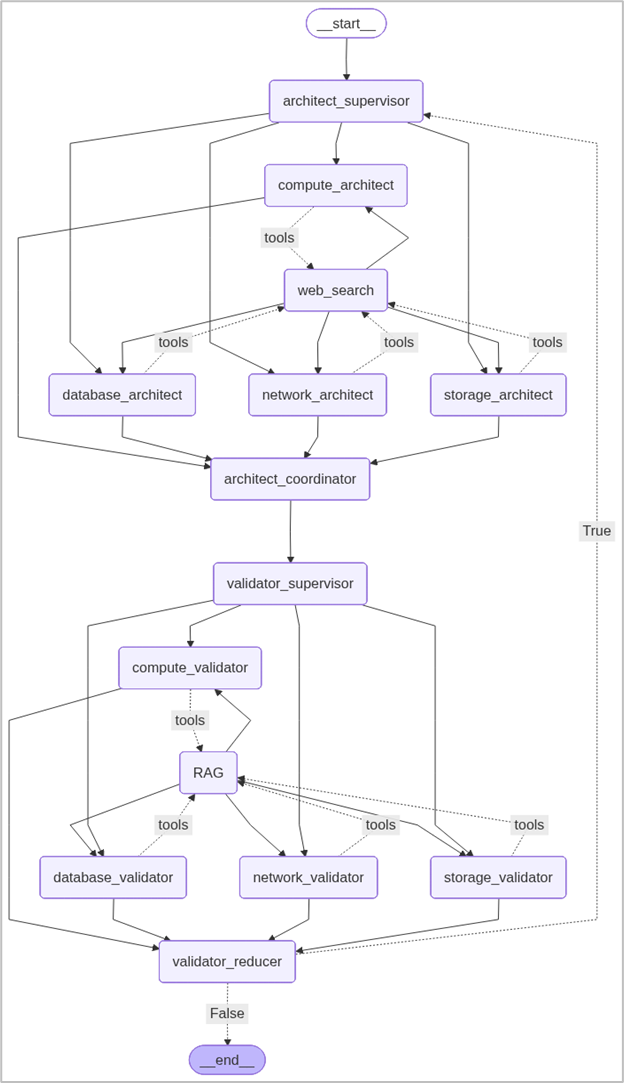
\includegraphics[width=0.7\textwidth]{LangGraphAgenticGraph.png}
\caption{Agent Framework Graph generated by LangGraph}
\label{fig:langgraph}
\end{figure}

\subsection{Supervisor Agent: Task Decomposition}

The \texttt{architectSupervisor} function/agent acts as the central orchestrator. It receives the initial user query describing architecture needs and decomposes it into structured, domain-specific tasks covering compute, network, storage, and database requirements. This agent incorporates feedback from validator agents to iteratively refine task definitions in subsequent cycles.

Error handling and retry mechanisms ensure robustness of LLM calls. The function produces a \texttt{State} object that holds the current tasks, iteration counts, and validation summaries, resetting or updating flags to control refinement loops. It uses the OpenAI GPT-4o reasoning model and generates structured output.

\subsection{Domain Architect Agents: Specialized Generation}

Functions/LangGraph nodes such as \texttt{computeArchitect}, \texttt{networkArchitect}, \texttt{storageArchitect}, and \texttt{databaseArchitect} implement domain-specific architect agents.

Each function/agent retrieves the task assigned by the supervisor—including requirements, constraints, and expected deliverables—and invokes the generator LLM equipped with web search. The agents produce detailed domain architecture drafts, recommending specific services (e.g., EC2, VPC, S3, RDS) and configurations.

Extensive validation ensures that agents respond with structured outputs. Error logging and fallback mechanisms handle incomplete or invalid responses gracefully. These agents use the OpenAI GPT-4o-mini model.

\subsection{Architecture Reducer Agent}

The \texttt{architectSynthesizer} function aggregates domain-specific recommendations into a unified architectural proposal. It acts as a synchronization node, merging outputs from parallel generation agents, maintaining consistency, and resolving potential conflicts. It uses the OpenAI GPT-4o reasoning model.

This step is vital for delivering a coherent end-to-end solution from independently generated domain components.

\subsection{Validation Supervisor Agent: Validation Task Decomposition}

The \texttt{validationSupervisor} function/agent orchestrates the validation process. It receives the initial user query, the generated architecture, and the structured domain-specific recommendations, then delegates validation tasks to the domain validator agents.

\subsection{Validator Agents}

The system employs \texttt{computeValidator}, \texttt{networkValidator}, \texttt{storageValidator}, and \texttt{databaseValidator} agents, each responsible for validating solutions against official AWS documentation cached in the vector database.

Validators utilize a Retrieval-Augmented Generation (RAG) approach, searching the ChromaDB vector embeddings created from parsed AWS documents and incorporating them into their reasoning process.

\subsection{Validation Reducer Agent}

Validation results are stored in the \texttt{validationFeedback} structure and analyzed by the \texttt{validationReducer} agent.

\subsection{Feedback Loop}

If any domain fails validation or reports factual inconsistencies, corrective feedback is sent to the supervisor agent, triggering another iteration of generation and synthesis.

This cyclical Evaluator–Optimizer feedback loop \cite{anthropic2024agents} is implemented as conditional edges in the LangGraph state graph, allowing a configurable number of refinement iterations or early termination upon successful validation.

\subsection{Final Architecture Generation}

Once all validations pass, or the maximum number of iterations is reached, the \texttt{finalArchitectureGenerator} function compiles a comprehensive architecture document. It includes executive summaries, detailed domain specifications, security considerations, cost optimization strategies, and deployment guidance.

The final document serves as a ready reference for system architects and stakeholders.

\section{Robustness Features}

The implementation incorporates robust error handling, retry logic with exponential backoff for LLM calls, and strict validation of responses to prevent the propagation of errors in multi-agent collaboration.

Timeouts, message filtering to avoid context bloat, and systematic logging support maintainability and traceability during iterative development and evaluation.

LangSmith is utilized for experiment tracking, debugging, and providing end-to-end observability across the multi-agent LLM workflow.